% =====================================================================
%  Rapport technique — Traducteur multilingue Francais / Anglais / Ewe
%  Projet GR02 — Master 1 IA-BD EPL S2
%
%  COMPILATION : XeLaTeX ou LuaLaTeX (PAS pdflatex).
%      xelatex gr_02_rapport_miagbe_traduction.tex ; xelatex gr_02_rapport_miagbe_traduction.tex   (2 passes pour la TdM)
%
%  Polices : famille DejaVu (.ttf du paquet TeX « dejavu »), couvre l'ewe.
%  Palette : inspiree du PowerPoint du projet (vert / or / rouge — Togo).
% =====================================================================
\documentclass[11pt,a4paper]{article}

\usepackage{fontspec}
\setmainfont{DejaVuSerif}[
  Extension=.ttf, UprightFont=*, BoldFont=*-Bold,
  ItalicFont=*-Italic, BoldItalicFont=*-BoldItalic, Scale=0.94]
\setsansfont{DejaVuSans}[
  Extension=.ttf, UprightFont=*, BoldFont=*-Bold,
  ItalicFont=*-Oblique, BoldItalicFont=*-BoldOblique, Scale=0.92]
\setmonofont{DejaVuSansMono}[
  Extension=.ttf, UprightFont=*, BoldFont=*-Bold,
  ItalicFont=*-Oblique, BoldItalicFont=*-BoldOblique, Scale=0.82]

\usepackage[french]{babel}
\usepackage[a4paper,top=2.6cm,bottom=2.6cm,left=2.5cm,right=2.5cm,headheight=0.8cm,headsep=0.5cm]{geometry}
\usepackage{graphicx}
\graphicspath{{images/}}
\usepackage{float}
\usepackage[table]{xcolor}
\usepackage{tikz}
\usepackage{booktabs}
\usepackage{tabularx}
\usepackage{array}
\usepackage{titlesec}
\usepackage{fancyhdr}
\usepackage{enumitem}
\usepackage{tcolorbox}
\usepackage{setspace}
\usepackage{url}
\usepackage[hidelinks]{hyperref}

% --- Interligne confortable -----------------------------------------
\setstretch{1.32}
\setlength{\parskip}{0.45em}
\setlength{\parindent}{0pt}

% --- Palette (PowerPoint du projet) ---------------------------------
\definecolor{primary}{HTML}{006A4E}      % vert principal
\definecolor{primarydark}{HTML}{14342F}  % vert tres fonce
\definecolor{gold}{HTML}{B38600}         % or fonce (lisible sur blanc)
\definecolor{goldbright}{HTML}{FFCE00}   % or vif (filets)
\definecolor{red}{HTML}{D21034}          % rouge accent
\definecolor{light}{HTML}{EAF7EF}        % fond encadre
\definecolor{lightline}{HTML}{DFE8E3}
\definecolor{greytxt}{HTML}{66746F}

\hypersetup{colorlinks=true,linkcolor=primary,urlcolor=primary}

% --- Chemins / code : police mono, coupables en bout de ligne -------
\DeclareUrlCommand\code{\urlstyle{tt}\def\UrlFont{\small\ttfamily\color{primarydark}}}

% --- Titres : carre vert numerote + titre vert (style maquette) -----
% Carre de taille fixe via un noeud TikZ (minimum size force largeur = hauteur ;
% les cles width/height de \tcbox etaient ignorees). Ajuster « minimum size »
% pour la taille du carre, et « baseline » pour l'alignement vertical au titre.
\newcommand{\secnum}[1]{%
  \tikz[baseline=-5pt]{%
    \node[fill=primary, rounded corners=3pt, minimum size=0.95cm,
          inner sep=0pt, anchor=center, text=white,
          font=\sffamily\bfseries\Large]{#1};}}

\titleformat{\section}[block]
  {\sffamily\LARGE\bfseries}
  {\secnum{\thesection}}{0.7em}{\color{primarydark}}
\titlespacing*{\section}{0pt}{0pt}{1.0em}

% Chaque grande partie commence sur une nouvelle page (rapport plus aere).
\newcommand{\sectionbreak}{\clearpage}

\titleformat{\subsection}
  {\sffamily\large\bfseries\color{primary}}
  {\textcolor{goldbright}{\rule[0.05em]{0.55em}{0.55em}}\ \thesubsection}{0.6em}{}
\titlespacing*{\subsection}{0pt}{1.1em}{0.4em}

% --- En-tete / pied avec logos --------------------------------------
\pagestyle{fancy}
\fancyhf{}
\fancyhead[L]{\footnotesize\sffamily\color{greytxt}Traducteur multilingue \textbullet{} FR \textbullet{} EN \textbullet{} ÉWÉ}
\fancyhead[R]{\footnotesize\sffamily\color{greytxt}Rapport technique}
\fancyfoot[L]{\footnotesize\sffamily\color{greytxt}Projet GR02 \textbullet{} INF2229}
\fancyfoot[R]{\footnotesize\sffamily\color{greytxt}\thepage}
\renewcommand{\headrulewidth}{1pt}
\renewcommand{\headrule}{\hbox to\headwidth{\color{primary}\leaders\hrule height 1pt\hfill}}
\renewcommand{\footrulewidth}{0.4pt}

% --- Encadres -------------------------------------------------------
\newtcolorbox{infobox}[1][]{colback=light,colframe=primary,boxrule=0.6pt,
  arc=3pt,left=10pt,right=10pt,top=7pt,bottom=7pt,
  fonttitle=\sffamily\bfseries\color{white},#1}
\newtcolorbox{keybox}[1][]{colback=white,colframe=gold,boxrule=1pt,
  arc=3pt,left=10pt,right=10pt,top=7pt,bottom=7pt,#1}

% =====================================================================
\begin{document}

% --------------------------- PAGE DE GARDE ---------------------------
\begin{titlepage}
\thispagestyle{empty}
\setstretch{1.05}

\noindent
\begin{minipage}[c]{0.46\textwidth}\raggedright
  
\includegraphics[height=1.85cm]{logo_epl.jpg}
\end{minipage}\hfill
\begin{minipage}[c]{0.46\textwidth}\raggedleft
  
\includegraphics[height=1.85cm]{logo_utbm.png}
\end{minipage}

\vspace{0.35cm}
\noindent{\color{primary}\rule{\textwidth}{1.4pt}}\\[-0.34cm]
\noindent{\color{goldbright}\rule{\textwidth}{0.6pt}}

\vfill
\begin{center}
{\sffamily\color{greytxt}\large Master 1 IA-BD — EPL}\\[0.18cm]
{\sffamily\color{greytxt}\large Cours INF2229 \textbullet{} Informatique et Gestion de Données}
\end{center}

\vfill
\begin{center}
{\sffamily\bfseries\color{primarydark}\fontsize{34}{38}\selectfont Traducteur Multilingue}\\[0.5cm]
{\sffamily\bfseries\color{primary}\LARGE FR \textbullet{} EN \textbullet{} ÉWÉ}\\[0.55cm]
{\sffamily\large\color{greytxt} avec reconnaissance et synthèse vocales}
\end{center}

\vspace{0.55cm}
\begin{center}
\tcbox[colback=primary, colframe=red, arc=6pt, boxrule=0pt,
       left=18pt, right=18pt, top=6pt, bottom=6pt, nobeforeafter]{%
  \sffamily\Large\bfseries\color{white} RAPPORT TECHNIQUE}
\end{center}

\vfill
\begin{center}
{\sffamily\bfseries\color{primary}\large Réalisé par — Groupe GR02}\\[0.28cm]
\begin{tcolorbox}[width=0.78\textwidth, colback=light, colframe=primary, arc=5pt, boxrule=0.7pt,
                  left=12pt, right=12pt, top=10pt, bottom=10pt, halign=center]
{\sffamily\setstretch{1.3}%
AZIGLOSSOU Judith Gracia \quad\textbullet\quad NAPO NISSAO Rafia\\
WOGLO Koffi Boris Gilbride \quad\textbullet\quad PIO Sikirou Afeez Prince Cyrille\\
KOMBATE Gountande\par}
\end{tcolorbox}
\vspace{0.4cm}
{\sffamily\bfseries\color{primary}\large Encadré par}\\[0.18cm]
{\sffamily\bfseries\color{primarydark} Dr. Akouyo Yvette GBEDEVI}{\sffamily\color{greytxt} }
\end{center}

\vfill
\noindent{\color{goldbright}\rule{\textwidth}{0.6pt}}\\[-0.34cm]
\noindent{\color{primary}\rule{\textwidth}{1.4pt}}
\begin{center}\sffamily\color{greytxt}\small Année universitaire 2025\,–\,2026\end{center}
\end{titlepage}

% --------------------------- RÉSUMÉ (page dédiée) --------------------
\section*{Résumé}
\addcontentsline{toc}{section}{Résumé}

Ce projet réalise un système de traduction automatique \textbf{multidirectionnel} entre
le français, l'anglais et l'éwé — langue gbe parlée au Togo et au Ghana, fortement
sous-dotée en ressources numériques. Le système couvre les \textbf{six} directions de
traduction possibles et il est complété d'une \textbf{chaîne vocale} de bout en bout
(reconnaissance et synthèse), l'éwé compris.

L'approche méthodologique privilégie le \textbf{transfert d'apprentissage} : plutôt que
d'entraîner un modèle depuis zéro, on adapte un grand modèle multilingue pré-entraîné,
\textbf{NLLB-200} de Meta, à l'aide d'un adaptateur \textbf{LoRA} (\emph{Low-Rank
Adaptation}). Le modèle est affiné sur un corpus trilingue de près de
\textbf{700\,000 paires} de phrases alignées, nettoyées et filtrées, puis enrichi par
\textbf{back-translation} : cette augmentation améliore nettement les directions vers
l'éwé et est retenue pour le modèle final.

L'évaluation, conduite à la fois sur un jeu interne et sur le jeu de référence
international \textbf{FLORES-200}, montre que l'adaptateur améliore les \textbf{six
directions sans aucune régression}, avec un gain moyen de \textbf{+1,24 point BLEU} et
\textbf{+1,64 point chrF} par rapport au modèle de base. La solution est exposée via une
API \textsc{FastAPI} et une interface web \textsc{React}.

\begin{infobox}
\textbf{Contribution principale.} Un traducteur trilingue opérationnel pour une langue
peu dotée, accompagné d'une méthodologie de données rigoureuse (alignement, filtrage,
contrôle du biais) et d'une évaluation honnête sur benchmark externe — démontrant un
apport mesurable du fine-tuning tout en documentant ses limites.
\end{infobox}

\clearpage

% --------------------------- SOMMAIRE (page dédiée) ------------------
{\hypersetup{linkcolor=primarydark}
 \renewcommand{\contentsname}{\sffamily\color{primarydark}Sommaire}
 \setcounter{tocdepth}{2}
 \begingroup\setstretch{1.0}\tableofcontents\endgroup}
\thispagestyle{fancy}
\clearpage

% =====================================================================
\section{Introduction et contexte}

\subsection{Problématique}
La traduction automatique a connu des progrès spectaculaires pour les langues dites
« à haute ressource » (anglais, français, etc.), mais les centaines de langues
africaines restent largement en marge de ces avancées. L'\textbf{éwé} (autonyme
\textit{Eʋegbe}), parlé par plusieurs millions de locuteurs au Togo et au Ghana, en est
un exemple représentatif : il dispose de très peu de corpus numériques, et les rares
données disponibles sont souvent bruitées, mal alignées, ou cantonnées à un domaine
unique (textes religieux notamment).

Ce projet s'attaque directement à ce déséquilibre en construisant un traducteur
couvrant les trois langues du sujet et leurs six directions, avec une attention
particulière portée à la \textbf{qualité des données} et à une \textbf{évaluation
rigoureuse} — les deux conditions sans lesquelles un score chiffré n'a pas de sens pour
une langue peu dotée.

\subsection{Objectifs}
Conformément au cahier des charges, le système couvre l'intégralité de la chaîne de
traitement :

\begin{itemize}[leftmargin=1.5em,itemsep=3pt]
  \item \textbf{Collecter} des corpus parallèles dans les trois langues à partir de
        sources ouvertes et de qualité contrôlée.
  \item \textbf{Prétraiter} les données : nettoyage, normalisation Unicode,
        tokenisation et alignement des phrases.
  \item \textbf{Entraîner} un modèle de traduction neuronale pour les paires
        Français~$\leftrightarrow$~Anglais, Français~$\leftrightarrow$~Éwé et
        Anglais~$\leftrightarrow$~Éwé.
  \item \textbf{Intégrer} une reconnaissance vocale (STT) et une synthèse vocale (TTS)
        pour la traduction orale.
  \item \textbf{Développer} une interface web permettant de tester le traducteur
        (saisie texte, dictée, écoute, historique).
\end{itemize}

\subsection{Choix de conception}
Trois décisions structurent l'ensemble du travail. Premièrement, le recours au
\textbf{transfert d'apprentissage} depuis un modèle massivement multilingue : c'est la
réponse recommandée par la littérature face au manque de données. Deuxièmement, la
priorité donnée au \textbf{nettoyage et au filtrage} du corpus, car sur une langue peu
dotée le bruit pèse davantage qu'un modèle plus gros. Troisièmement, une
\textbf{évaluation sur benchmark externe} (FLORES-200) afin d'obtenir des chiffres
comparables et honnêtes, et non flattés par la proximité au domaine d'entraînement.

% =====================================================================
\section{Architecture générale}

Le projet est organisé en quatre blocs indépendants et reproductibles, qui se
transmettent leurs sorties par fichiers. Cette séparation permet de relancer une étape
sans rejouer les précédentes, et de tracer précisément l'origine de chaque résultat.

\begin{enumerate}[leftmargin=1.6em,itemsep=4pt]
  \item \textbf{Construction des données} — \code{notebooks/00_donnees.ipynb}. Collecte,
        nettoyage, alignement, filtrage et découpage. Produit le corpus final dans
        \code{data/processed/nllb/} (fichiers \code{nllb_train.csv}, \code{nllb_valid.csv},
        \code{nllb_test.csv}).
  \item \textbf{Modèle de traduction} — \code{notebooks/01_pipeline_nllb_lora.ipynb}.
        Fine-tuning LoRA de NLLB-200, suivi des pertes, évaluation BLEU/chrF et
        comparaison base vs adaptateur sur FLORES-200.
  \item \textbf{Augmentation} — \code{notebooks/02_backtranslation_nllb_lora.ipynb}.
        Génération de données synthétiques par back-translation, ré-entraînement dans un
        dossier séparé et comparaison systématique avant adoption.
  \item \textbf{Service applicatif} — \code{src/traducteur/}. API \textsc{FastAPI}
        (endpoints de traduction, transcription, synthèse, historique) et interface
        \textsc{React}/\textsc{Vite}.
\end{enumerate}

\begin{infobox}
\textbf{Pile technologique.} Python, PyTorch, Hugging Face Transformers et PEFT pour le
modèle ; \texttt{sacrebleu} pour l'évaluation ; \texttt{librosa}, Whisper et MMS pour
l'audio ; FastAPI (backend) et React/Vite (frontend) ; Git/GitHub pour la
collaboration. Ces choix correspondent aux technologies recommandées par le sujet.
\end{infobox}

% =====================================================================
\section{Construction du corpus}

La qualité du corpus est le facteur déterminant pour une langue peu dotée. Le notebook
de données enchaîne sept étapes, de la collecte au bilan final.

\subsection{Sources}
Le corpus combine plusieurs jeux ouverts, choisis pour leur licence et leur niveau de
qualité, et répartis en deux familles :

\begin{itemize}[leftmargin=1.5em,itemsep=3pt]
  \item \textbf{Sources « propres » (humaines)} : \textbf{google/SMOL} (traductions
        professionnelles en–ee), \textbf{FLORES} (découpage \code{dev}, aligné dans les
        trois langues), \textbf{MAFAND} (fr–ewe, actualités, projet Masakhane). Elles
        entrent directement dans le corpus.
  \item \textbf{Sources web-minées} : OPUS (NLLB, TED2020, Tatoeba, News-Commentary,
        translatewiki) et une part biblique. Plus volumineuses mais plus bruitées, elles
        passent par tout le pipeline de durcissement décrit ci-dessous.
\end{itemize}

Toutes ces sources sont des \textbf{données secondaires} : des corpus publics déjà
constitués par des tiers. Le projet ne réalise pas de collecte \emph{primaire} (ni
scraping de nouveaux sites, ni enregistrements) — c'est la voie « bases de données
ouvertes » prévue par le cahier des charges. Trois canaux d'accès sont utilisés : le
dépôt \textbf{OPUS} (\texttt{opus.nlpl.eu}, téléchargement direct), la bibliothèque
\textbf{Hugging Face \texttt{datasets}}, et \textbf{GitHub}.

\begin{table}[H]
\centering\small
\setstretch{1.1}
\renewcommand{\arraystretch}{1.2}
\begin{tabularx}{\textwidth}{l l X l}
\toprule
\rowcolor{light}
\textbf{Source} & \textbf{Langues} & \textbf{Producteur / nature} & \textbf{Accès} \\
\midrule
OPUS-NLLB            & ee–fr, en–ee & Meta — bitexte miné du web      & OPUS \\
OPUS-bible-uedin     & ee–en, ee–fr & traductions bibliques           & OPUS \\
OPUS-TED2020         & en–fr        & sous-titres TED (humain)        & OPUS \\
OPUS-Tatoeba         & en–fr        & phrases communautaires          & OPUS \\
OPUS-News-Commentary & en–fr        & commentaires d'actualité        & OPUS \\
OPUS-translatewiki   & ee–fr        & localisation logicielle         & OPUS \\
google/SMOL          & en–ee        & Google — traductions pro.       & HF Hub \\
FLORES-200 (dev)     & fr/en/ewe    & Meta — benchmark aligné (éval)  & HF Hub \\
MAFAND (lafand-mt)   & fr–ewe       & Masakhane — actualités          & GitHub \\
\bottomrule
\end{tabularx}
\caption{Provenance des sources. Toutes sont publiques et citables ; le corpus Ghana NLP (en–ewe, biblique) a été écarté pour cause de biais.}
\end{table}

L'apport du projet n'est donc pas la collecte brute, mais l'\textbf{ingénierie de
données} : agrégation, alignement, filtrage et contrôle du biais (sections suivantes).

\subsection{Nettoyage et normalisation}
Chaque phrase est nettoyée (suppression des caractères de contrôle et des artefacts de
balisage), puis \textbf{normalisée en Unicode} afin d'unifier les multiples
représentations possibles des caractères éwé accentués et des signes diacritiques. Cette
normalisation est essentielle : sans elle, deux occurrences visuellement identiques d'un
même mot éwé peuvent être encodées différemment et fausser à la fois l'apprentissage et
l'évaluation.

\subsection{Alignement et filtrage du bruit}
Les paires web-minées subissent un filtrage en plusieurs passes :

\begin{enumerate}[leftmargin=1.5em,itemsep=3pt]
  \item \textbf{Alignement par similarité cosinus.} Chaque phrase est encodée par
        l'encodeur de NLLB ; on ne conserve une paire que si la similarité cosinus entre
        la source et la cible dépasse un seuil. Cela élimine les paires mal appariées.
  \item \textbf{Identification de langue (LID).} Un filtre fastText (modèle NLLB-LID)
        écarte les phrases dans la mauvaise langue. La LID seule étant peu fiable sur
        l'éwé en textes courts, elle est \textbf{complétée d'une heuristique de
        caractères éwé} : on vérifie la présence de lettres propres à la langue
        (\mbox{ɖ\,ƒ\,ŋ\,ɔ\,ɛ\,ɣ\,ʋ}), ce qui réduit fortement la confusion avec l'anglais.
  \item \textbf{Déduplication} des paires identiques, puis \textbf{durcissement du seuil}
        cosinus sur les sources les plus bruitées avant la construction finale.
\end{enumerate}

\subsection{Tokenisation}
La tokenisation n'est pas réimplémentée : elle est déléguée au tokenizer
\textbf{SentencePiece} de NLLB, un modèle de sous-mots de type \emph{unigram}. Ce choix
est cohérent avec le modèle utilisé et présente deux avantages décisifs pour l'éwé :
il ne dépend pas du découpage par espaces, et il gère les mots inconnus en les
décomposant en sous-unités. La langue source et la langue cible sont injectées
directement dans la tokenisation au moyen des codes \code{fra_Latn}, \code{eng_Latn} et
\code{ewe_Latn}, ce qui permet au même modèle de traiter les six directions.

\subsection{Découpage et volumétrie}
Le corpus est découpé en \code{train}/\code{valid}/\code{test} une fois pour toutes, et
ce découpage est \textbf{réutilisé à l'identique} dans toutes les expériences : aucune
phrase du test ou de la validation n'apparaît à l'entraînement, ce qui garantit
l'absence de fuite et la comparabilité des scores.

\textbf{L'entonnoir de données} résume les volumes à chaque étape : plus de deux millions
de paires candidates ont été traitées, ramenées à environ un million de paires
\emph{exploitables} après filtrage, puis volontairement \textbf{plafonnées} pour
équilibrer les six directions. La quantité visée n'est pas le volume brut mais une
quantité \emph{propre et équilibrée}.

\begin{table}[H]
\centering\small
\setstretch{1.1}
\renewcommand{\arraystretch}{1.2}
\begin{tabular}{l r}
\toprule
\rowcolor{light}
\textbf{Étape} & \textbf{Paires} \\
\midrule
Collecté / traité (toutes sources) & $\approx$ 2\,000\,000 \\
Après alignement cosinus, LID et filtre éwé & 1\,090\,357 \\
Après filtres anti-bruit & 1\,088\,846 \\
Après déduplication & 1\,064\,356 \\
Bidirectionnalisation ($\times 2$) & 2\,128\,712 \\
\textbf{Après plafond de 120\,000 / direction} & \textcolor{primary}{\textbf{697\,744}} \\
\midrule
\multicolumn{2}{l}{\itshape dont train 669\,904 \textbullet{} validation 13\,853 \textbullet{} test 13\,987} \\
\bottomrule
\end{tabular}
\caption{Entonnoir de données : du brut collecté au corpus final équilibré. Environ 1,4 million de paires \emph{exploitables} ont été écartées par choix d'équilibrage (plafond par direction).}
\end{table}

\begin{table}[H]
\centering\small
\setstretch{1.1}
\renewcommand{\arraystretch}{1.2}
\begin{tabular}{l r r r r r r r}
\toprule
\rowcolor{light}
\textbf{Split} & \textbf{EN→EWE} & \textbf{EN→FR} & \textbf{EWE→EN} & \textbf{EWE→FR} & \textbf{FR→EN} & \textbf{FR→EWE} & \textbf{Total} \\
\midrule
Train & 104\,499 & 115\,223 & 104\,499 & 115\,184 & 115\,223 & 115\,276 & \textbf{669\,904} \\
\addlinespace
\multicolumn{8}{l}{\itshape Validation : 13\,853 paires \quad\textbullet\quad Test : 13\,987 paires} \\
\bottomrule
\end{tabular}
\caption{Volumétrie du corpus trilingue final. Les six directions sont volontairement équilibrées.}
\end{table}

\subsection{Contrôle du biais}
Un risque majeur sur l'éwé est le \textbf{biais de domaine biblique} : une grande partie
des corpus disponibles provient de traductions religieuses, dont le vocabulaire et le
style ne reflètent pas la langue courante. Deux mesures l'atténuent : chaque paire porte
un drapeau \code{is_religious} permettant de quantifier et de plafonner cette part
(limitée à \textbf{36\,530} lignes au train, soit environ \textbf{5,5\,\%}) ; et le
corpus \textbf{Ghana NLP} (en–ewe, d'origine essentiellement biblique et fortement
biaisé) a été \textbf{écarté} du jeu final.

% =====================================================================
\section{Modèle de traduction}

\subsection{Modèle de base : NLLB-200}
Le système s'appuie sur \textbf{\code{facebook/nllb-200-distilled-600M}}, une version
distillée (600 millions de paramètres) du modèle \textit{No Language Left Behind} de
Meta. C'est un Transformer encodeur–décodeur entraîné sur 200 langues, dont l'éwé. La
version distillée offre le meilleur compromis entre qualité et coût : elle tient sur un
seul GPU grand public et reste rapide en inférence, ce qui est indispensable pour une
application interactive.

\subsection{Adaptation par LoRA}
Affiner les 600 millions de paramètres serait coûteux et risquerait l'oubli
catastrophique des connaissances multilingues du modèle. On emploie donc \textbf{LoRA}
(\emph{Low-Rank Adaptation}) : on \textbf{gèle entièrement} le modèle de base et on
n'apprend que de petites matrices de rang faible, insérées dans les couches d'attention
et les couches \emph{feed-forward}. Seuls quelques pour cent des paramètres sont
entraînés, ce qui réduit massivement la mémoire et le temps de calcul, tout en
préservant le socle pré-entraîné. La matrice d'embedding et la tête de sortie restent
gelées : la tokenisation et les représentations de NLLB ne sont donc pas dégradées.

\begin{table}[H]
\centering\small
\setstretch{1.1}
\renewcommand{\arraystretch}{1.25}
\begin{tabularx}{\textwidth}{>{\bfseries\color{primary}}l X}
\toprule
\rowcolor{light}\textbf{Hyperparamètre} & \textbf{Valeur et justification} \\
\midrule
Modèle de base & \code{facebook/nllb-200-distilled-600M} (encodeur–décodeur, 200 langues). \\
Rang LoRA & $r=32$, $\alpha=64$, dropout $0{,}05$ — capacité suffisante pour apprendre à générer l'éwé. \\
Modules adaptés & \code{q_proj, k_proj, v_proj, out_proj, fc1, fc2} — attention \emph{et} feed-forward. \\
Époques & 2 (soit 6\,250 pas) — au-delà, la perte de validation plafonne. \\
Lot effectif & 64 (32 $\times$ 2 accumulations de gradient). \\
Taux d'apprentissage & $2\times10^{-4}$, avec \emph{warmup} de 3\,\%. \\
Précision & bf16 + \emph{gradient checkpointing} pour tenir en mémoire GPU. \\
Longueur de séquence & 128 tokens en source et en cible. \\
Sélection & \emph{load best model} : on conserve le point de contrôle de meilleure \code{eval_loss}. \\
\bottomrule
\end{tabularx}
\caption{Configuration d'entraînement de l'adaptateur LoRA et justifications.}
\end{table}

\subsection{Dynamique d'entraînement}
La perte de validation décroît de façon \textbf{monotone} tout au long des deux époques,
sans aucun rebond — signe d'une bonne généralisation et de l'absence de sur-apprentissage.
Elle baissait encore légèrement en fin d'entraînement, ce qui suggère une marge
résiduelle (cf. perspectives). Le mécanisme \emph{load best model} garantit que l'on
conserve le meilleur état même en cas de léger sur-apprentissage tardif.

\begin{table}[H]
\centering\small
\setstretch{1.1}
\renewcommand{\arraystretch}{1.2}
\begin{tabular}{r r r}
\toprule
\rowcolor{light}\textbf{Pas} & \textbf{Époque} & \textbf{Perte de validation} \\
\midrule
1\,000 & 0,32 & 1,1487 \\
3\,000 & 0,96 & 1,1273 \\
5\,000 & 1,60 & 1,1184 \\
6\,250 & 2,00 & \textbf{1,1165} \\
\bottomrule
\end{tabular}
\caption{Décroissance régulière de la perte de validation (extraits).}
\end{table}

\subsection{Augmentation par back-translation}
Pour renforcer les directions \emph{vers l'éwé}, les plus pauvres en données, on applique
la \textbf{back-translation}. Le principe : conserver l'\textbf{éwé humain en cible} (donc
de qualité garantie) et fabriquer une \textbf{source synthétique} à l'aide du modèle déjà
entraîné, uniquement à partir des paires propres \code{(ewe, fr)} du train. Trois jeux
sont produits :

\begin{itemize}[leftmargin=1.5em,itemsep=3pt]
  \item \textbf{A} (\code{fr}~$\to$~\code{en}) : génère des paires
        \code{en_synth}~$\to$~\code{ewe} et enrichit ainsi la direction EN→EWE en contenu
        varié et non biblique.
  \item \textbf{A2} (réutilisation) : le même anglais synthétique sert à créer
        \code{ewe}~$\to$~\code{en_synth}, ce qui équilibre EWE→EN sans calcul GPU
        supplémentaire.
  \item \textbf{B} (\code{ewe}~$\to$~\code{fr}) : génère des paires
        \code{fr_synth}~$\to$~\code{ewe} pour renforcer FR→EWE et réduire l'\emph{off-target}
        (sortie en mauvaise langue).
\end{itemize}

Seules les cibles éwé \textbf{pristines} (similarité cosinus élevée \emph{et} présence de
caractères éwé) alimentent ce processus, afin de ne pas injecter de bruit. Le modèle
augmenté est entraîné dans un dossier distinct, puis \textbf{comparé} au modèle sans
augmentation selon une \textbf{règle d'adoption stricte} : ne retenir la back-translation
que si elle améliore en$\leftrightarrow$ewe \emph{sans} régresser ailleurs. Les résultats
de cette comparaison sont présentés dans la section \emph{Évaluation}.

% =====================================================================
\section{Évaluation}

\subsection{Métriques}
Deux métriques complémentaires sont utilisées via la bibliothèque \texttt{sacrebleu} :

\begin{itemize}[leftmargin=1.5em,itemsep=3pt]
  \item \textbf{BLEU} mesure le recouvrement de n-grammes de \emph{mots} entre la
        prédiction et la référence. C'est la métrique historique, comparable à la
        littérature.
  \item \textbf{chrF} mesure le recouvrement de n-grammes de \emph{caractères}. Elle est
        particulièrement pertinente pour l'éwé, langue à morphologie riche et à
        diacritiques, où une métrique au mot pénalise injustement de petites variations.
\end{itemize}

La génération utilise une recherche en faisceau (\emph{beam search}) à 4 faisceaux.

\subsection{Protocole}
L'évaluation est conduite sur deux jeux, par direction :

\begin{itemize}[leftmargin=1.5em,itemsep=3pt]
  \item \textbf{Test interne} (\code{nllb_test.csv}) : issu de la même distribution que
        l'entraînement. Utile, mais \textbf{optimiste}.
  \item \textbf{FLORES-200} (\code{devtest}) : jeu de référence multilingue de Meta,
        \textbf{jamais vu} à l'entraînement et aligné dans les trois langues. C'est la
        mesure \textbf{honnête} et comparable à l'état de l'art, y compris pour
        en$\leftrightarrow$ewe.
\end{itemize}

\subsection{Résultat principal : base vs LoRA sur FLORES-200}
La comparaison oppose le NLLB de base (adaptateur désactivé) à notre adaptateur LoRA, sur
exactement les mêmes phrases. L'adaptateur \textbf{améliore les six directions}. Ces
scores mesurent l'apport du fine-tuning (NLLB $\to$ LoRA) ; le modèle final y ajoute la
\textbf{back-translation} (présentée plus haut), qui renforce encore les directions vers
l'éwé — sa mesure sur FLORES reste une perspective.

\begin{figure}[H]
\centering
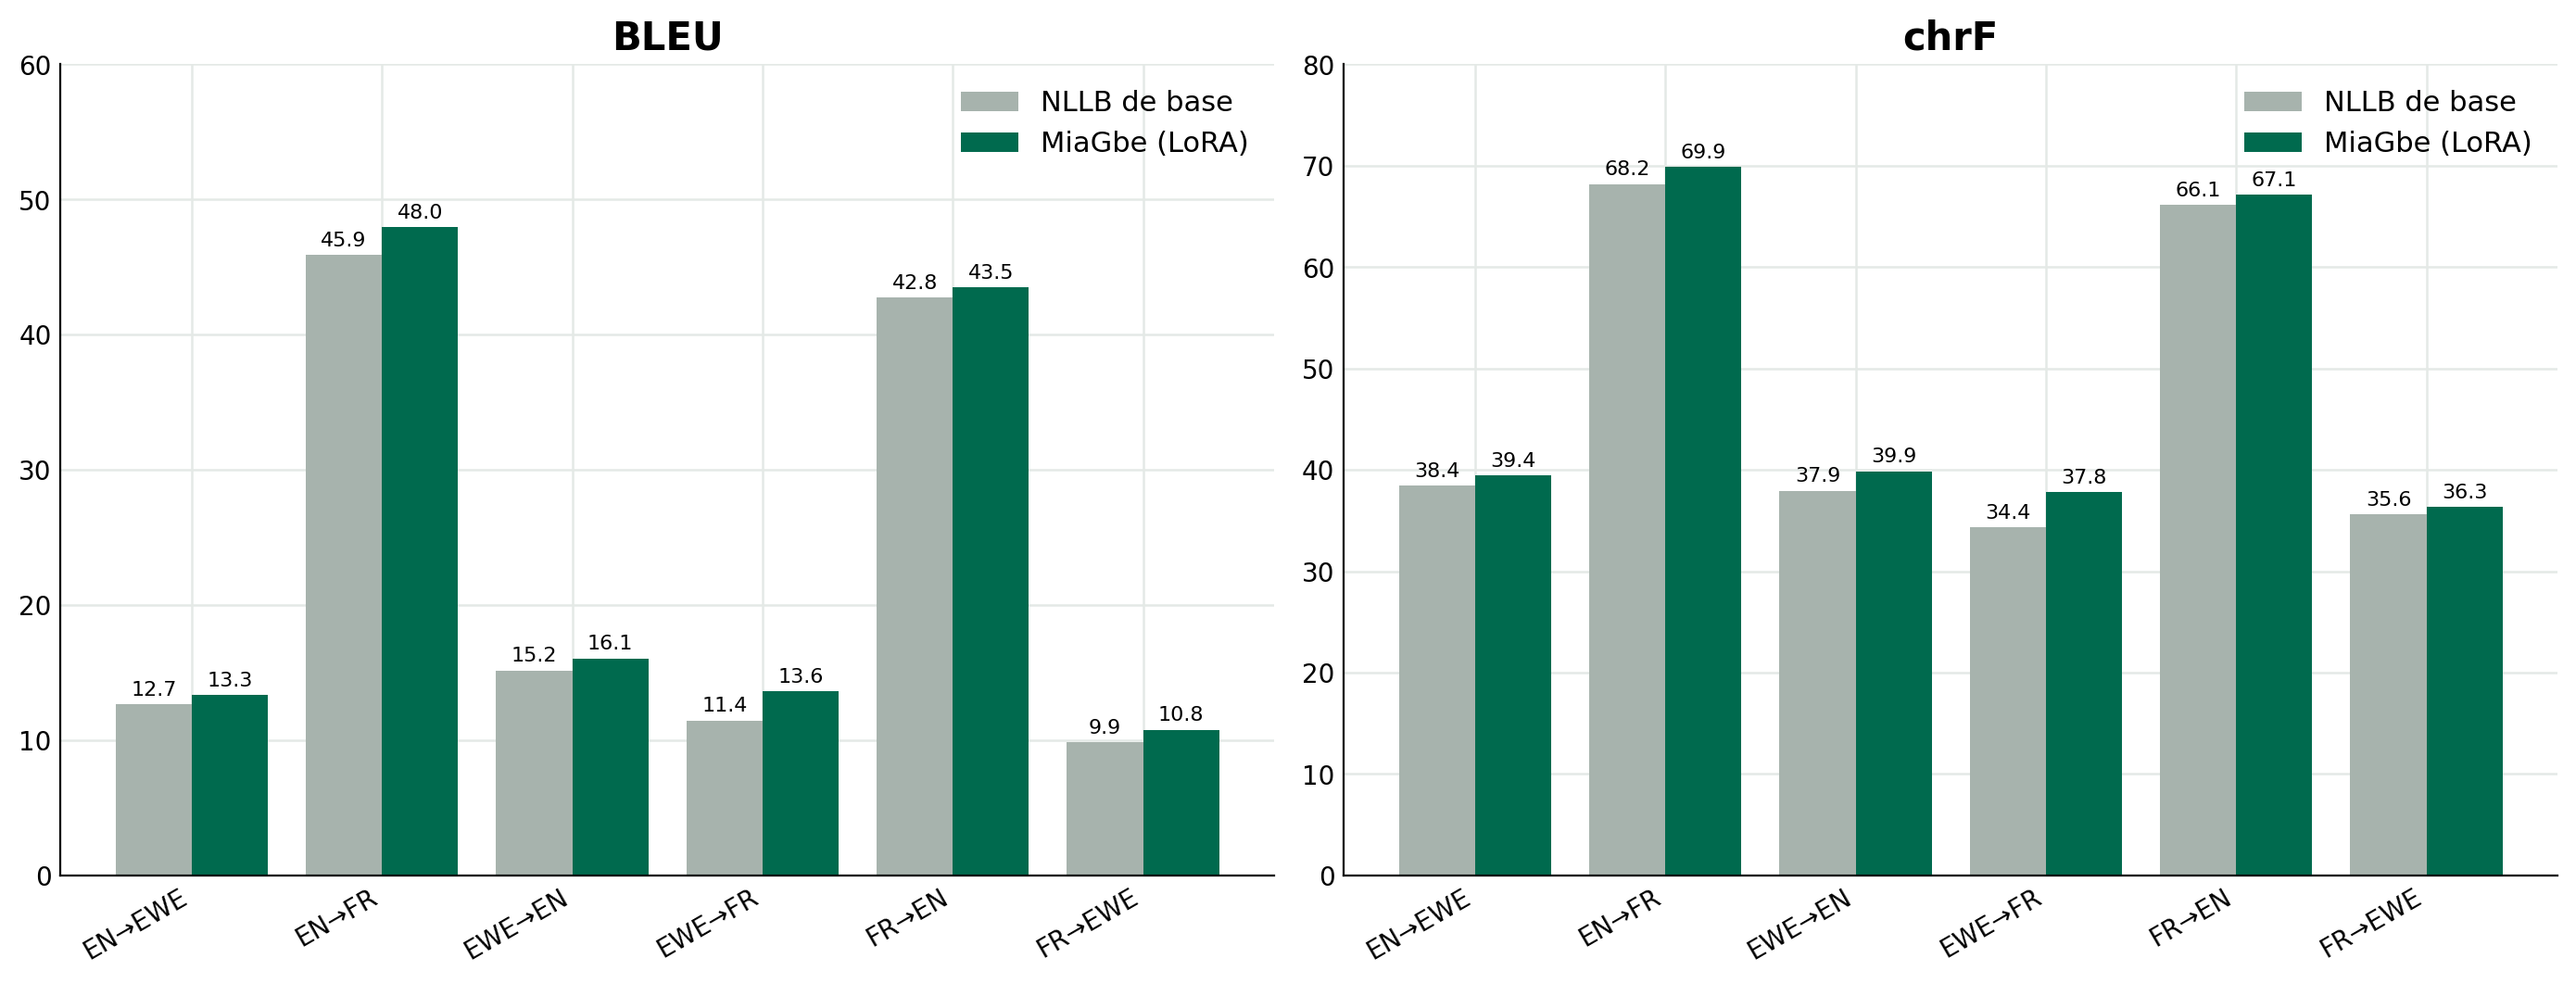
\includegraphics[width=\textwidth]{charts/flores.png}
\caption{FLORES-200 \texttt{devtest} : NLLB de base vs MiaGbe (BLEU et chrF, 200 phrases par direction). Le fine-tuning améliore les six directions ; moyenne +1,24 BLEU et +1,64 chrF.}
\end{figure}

\subsection{Test interne}
\begin{figure}[H]
\centering
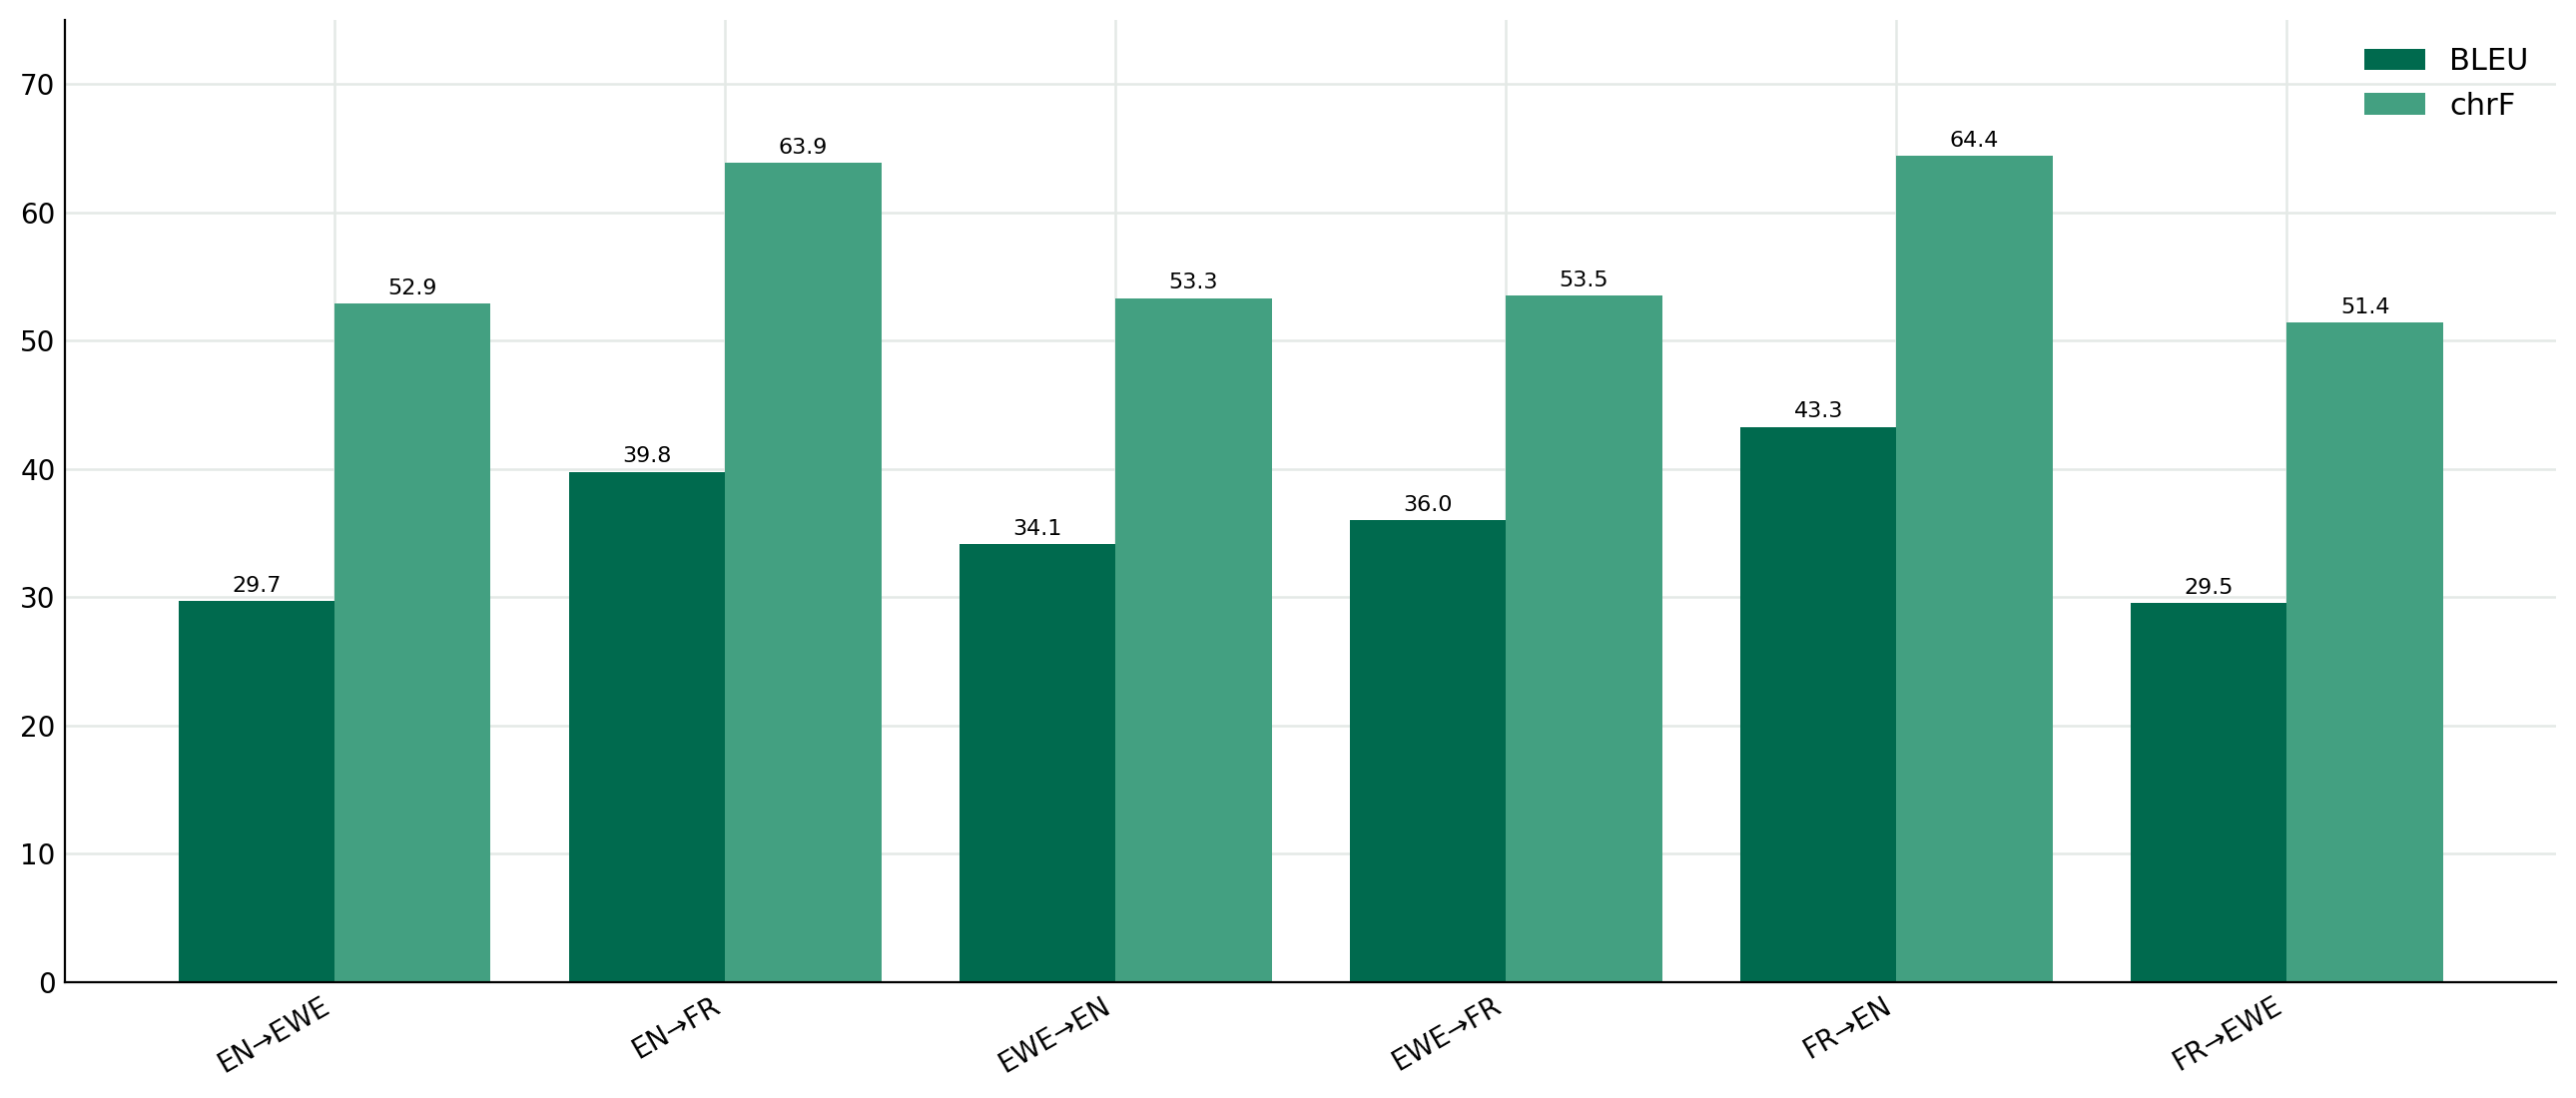
\includegraphics[width=\textwidth]{charts/internal.png}
\caption{Scores du modèle LoRA sur le test interne, issu de nos données (BLEU et chrF par direction ; avant back-translation). La back-translation relève encore les directions vers l'éwé.}
\end{figure}

\subsection{Apport de la back-translation}
La règle d'adoption (gagner sur en$\leftrightarrow$ewe sans régresser ailleurs) est
\textbf{vérifiée} : les directions vers l'éwé progressent nettement — EN→EWE \textbf{+3,1}
BLEU et FR→EWE \textbf{+1,4} BLEU — tandis que les autres restent stables. La
back-translation est donc \textbf{retenue pour le modèle final}.

\begin{figure}[H]
\centering
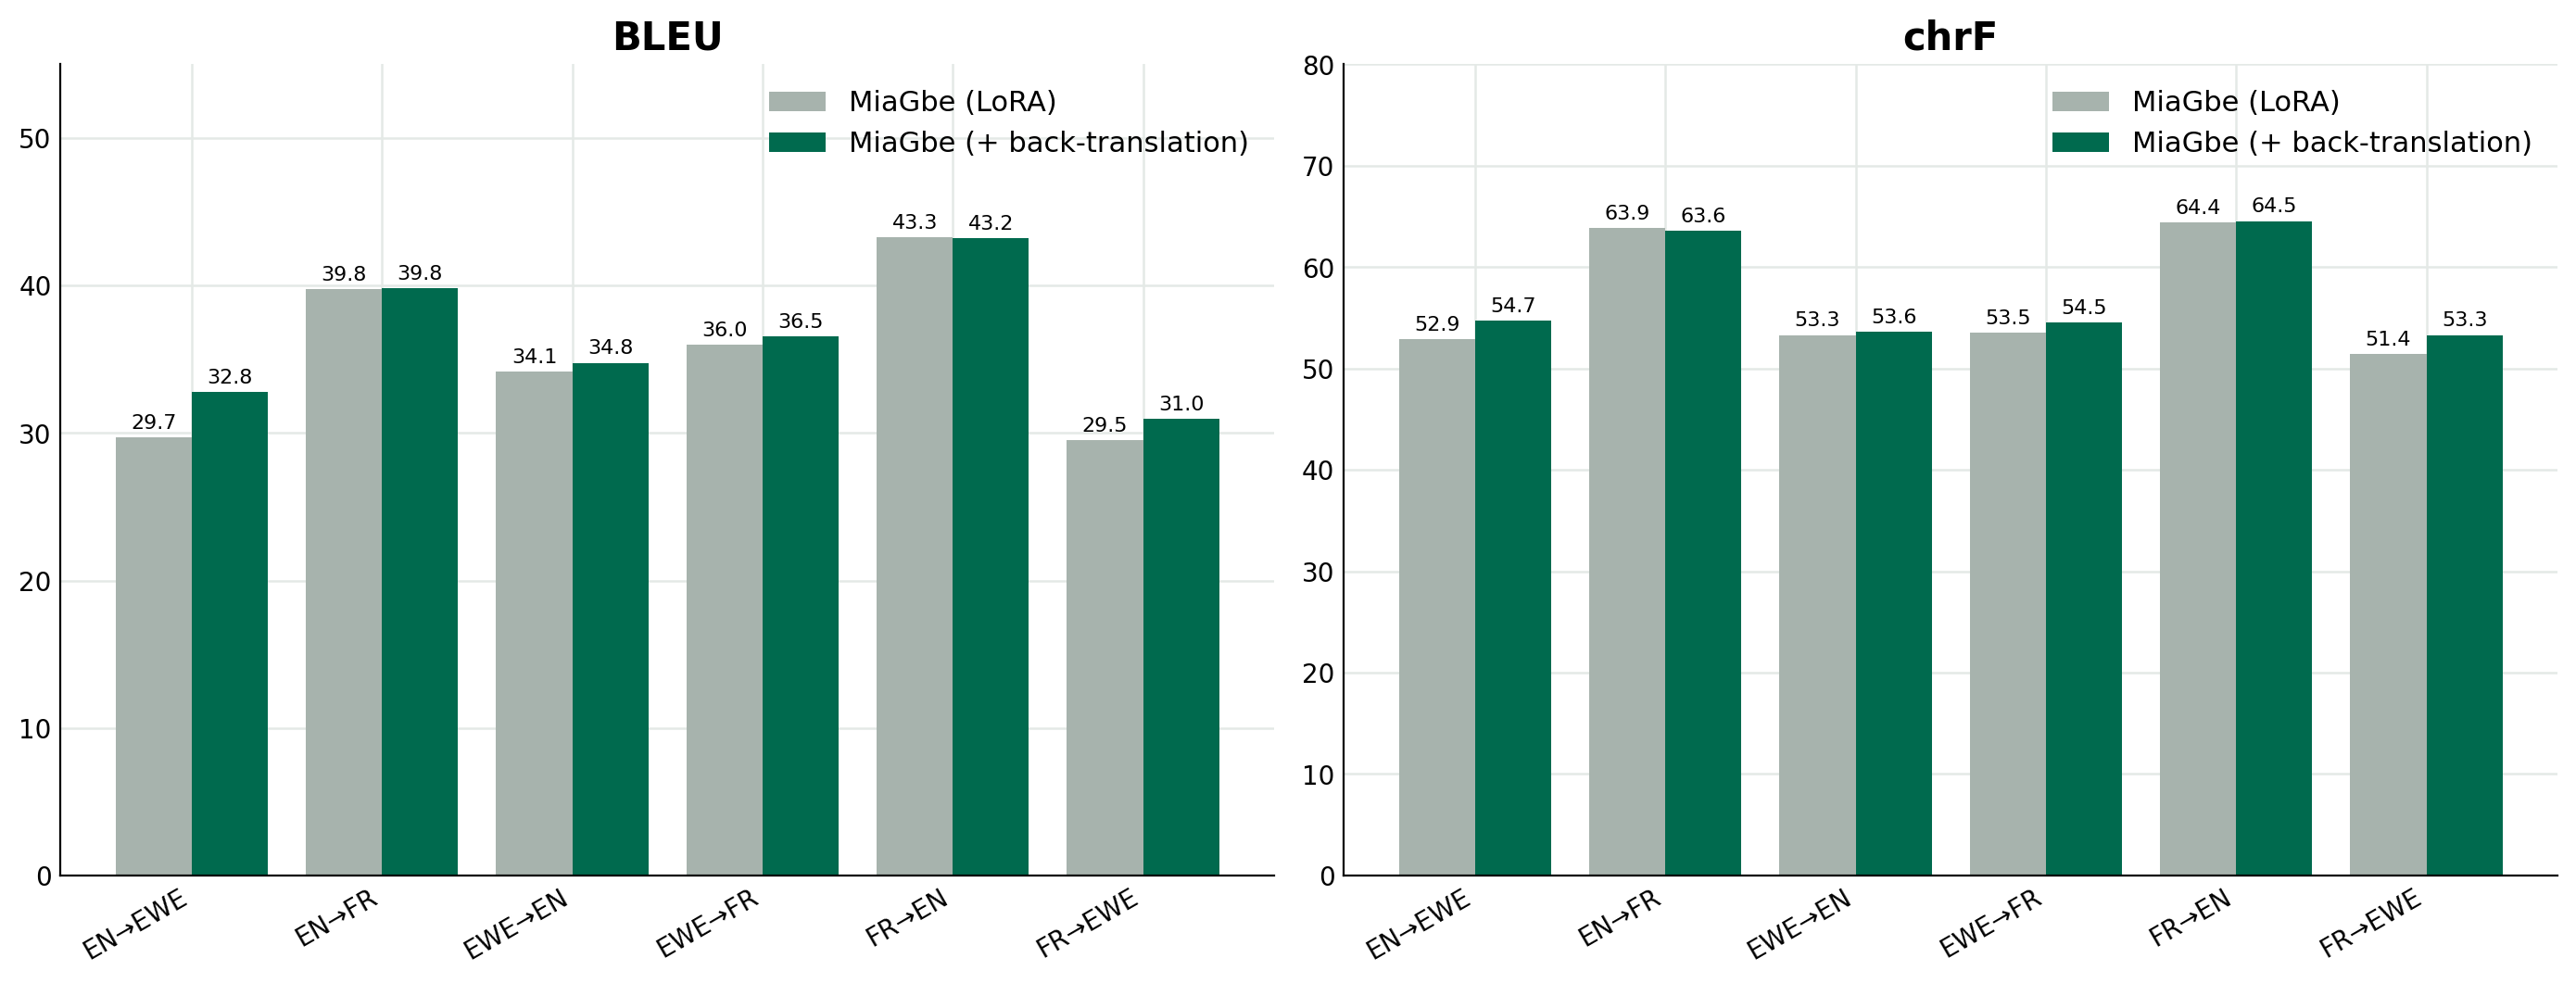
\includegraphics[width=\textwidth]{charts/bt.png}
\caption{Apport de la back-translation : adaptateur LoRA seul vs LoRA + back-translation, sur le test interne (BLEU et chrF). Les directions vers l'éwé progressent nettement (EN→EWE +3,1 ; FR→EWE +1,4 BLEU), sans régression ailleurs.}
\end{figure}

\emph{Réserve d'honnêteté} : ce gain est mesuré sur le test interne (optimiste) ; sa
confirmation sur FLORES-200 reste une étape à mener.

\subsection{Analyse}
\begin{itemize}[leftmargin=1.5em,itemsep=4pt]
  \item \textbf{Aucune régression.} Sur le benchmark externe, le fine-tuning aide les six
        directions à la fois (+1,24 BLEU et +1,64 chrF en moyenne). C'est le résultat le
        plus solide et le plus défendable du projet.
  \item \textbf{Back-translation décisive.} Sur le test interne, l'augmentation gagne
        \textbf{+3,1 BLEU} en EN→EWE et \textbf{+1,4} en FR→EWE, sans régression ailleurs :
        c'est ce qui justifie son adoption pour le modèle final.
  \item \textbf{Écart test interne / FLORES.} Pour un même modèle (LoRA), FR→EWE atteint
        29,5 BLEU en interne mais seulement 10,8 sur FLORES. Cet écart, attendu, illustre
        pourquoi un test proche du domaine d'entraînement est trompeur : seul FLORES donne
        une mesure réaliste de la généralisation.
  \item \textbf{Génération vers l'éwé.} Sur FLORES, les directions $\to$EWE progressent le
        moins (+0,69 et +0,90 BLEU) et restent basses en valeur absolue — conséquence de la
        rareté des cibles éwé de qualité. La back-translation les renforce nettement, et
        reste le principal axe d'amélioration.
\end{itemize}

\begin{keybox}
\textbf{Exemple qualitatif} (EN→EWE).\\
Source : \textit{« Vatican City's population is around 800. »}\\
Sortie du modèle : \textit{« Vatika dukɔ ƒe agbɔsɔsɔ nye 800. »}\\
La sortie est une phrase éwé bien formée, employant correctement les caractères
spécifiques de la langue.
\end{keybox}

% =====================================================================
\section{Chaîne vocale}

La chaîne vocale couvre les trois langues sans dépendance à un outil externe comme
\texttt{ffmpeg} : le navigateur enregistre directement en WAV, décodé côté serveur par
\texttt{librosa} (rééchantillonnage à 16 kHz, mono).

\begin{itemize}[leftmargin=1.5em,itemsep=3pt]
  \item \textbf{Reconnaissance vocale (STT).} \textbf{Whisper} (OpenAI) pour le français
        et l'anglais ; \textbf{MMS-ASR} (Meta, fondé sur Wav2Vec2 et couvrant plus de
        1\,100 langues) pour l'\textbf{éwé}, via son adaptateur de langue dédié.
  \item \textbf{Synthèse vocale (TTS).} \textbf{MMS-TTS} (Meta) pour l'éwé, que les
        navigateurs ne savent pas prononcer ; la voix native du navigateur pour le
        français et l'anglais.
\end{itemize}

\begin{infobox}
\textbf{Optimisations de performance:} L'inférence audio s'exécute sur GPU détecté
automatiquement ; les modèles sont \textbf{préchargés au démarrage} du serveur (ce qui
élimine la latence du premier appel) ; l'adaptateur de langue MMS est mis en cache pour
ne pas être rechargé à chaque requête ; et la transcription s'exécute hors de la boucle
asynchrone, afin de ne pas bloquer le service.
\end{infobox}

% =====================================================================
\section{Interface et API}

Le backend \textsc{FastAPI} expose des endpoints clairs : \code{/translate} (traduction
texte), \code{/transcribe} (reconnaissance vocale), \code{/synthesize} (synthèse vocale)
et \code{/history} (historique). Le modèle de traduction et les modèles audio y sont
chargés une seule fois et réutilisés.

L'interface \textsc{React}/\textsc{Vite} offre les fonctionnalités demandées par le
cahier des charges :

\begin{itemize}[leftmargin=1.5em,itemsep=3pt]
  \item \textbf{Saisie texte} avec traduction quasi instantanée (déclenchée après une
        courte pause de frappe).
  \item \textbf{Dictée vocale} : enregistrement puis transcription côté serveur, unifiée
        pour les trois langues, avec un indicateur visuel de l'état (enregistrement,
        puis transcription en cours).
  \item \textbf{Écoute} de la traduction par synthèse vocale.
  \item \textbf{Historique} des traductions, synchronisé côté serveur entre navigateurs
        (authentification Google optionnelle).
\end{itemize}

% =====================================================================
\section{Limites et perspectives}

\subsection{Limites}
\begin{itemize}[leftmargin=1.5em,itemsep=3pt]
  \item \textbf{Génération vers l'éwé} : c'est le maillon faible (BLEU FLORES de l'ordre
        de 10 à 13). La disponibilité de cibles éwé de qualité reste le facteur limitant.
  \item \textbf{Hétérogénéité des données} : malgré le filtrage, une part de contenu
        biblique subsiste et le style global demeure inégal.
  \item \textbf{Couverture audio de l'éwé} : la qualité du STT/TTS éwé dépend des modèles
        MMS pré-entraînés, non affinés sur des locuteurs spécifiques.
\end{itemize}

\subsection{Perspectives}
\begin{itemize}[leftmargin=1.5em,itemsep=3pt]
  \item Confirmer le gain de la back-translation sur FLORES-200 (benchmark externe).
  \item Prolonger l'entraînement (la perte de validation baissait encore en fin de course).
  \item Étendre la back-translation EN→EWE à plus grande échelle.
  \item Augmenter le rang LoRA sur le décodeur pour accroître la capacité de génération.
  \item Collaborer avec des locuteurs natifs pour annoter du contenu courant — le levier
        le plus efficace à long terme pour une langue peu dotée.
\end{itemize}

% =====================================================================
\section{Conclusion}

Le projet livre un traducteur \textbf{trilingue opérationnel} sur les six directions,
fondé sur le fine-tuning LoRA de NLLB-200, un corpus de près de 700\,000 paires
soigneusement filtrées et une augmentation par back-translation. Sur le benchmark externe
FLORES-200, l'adaptateur \textbf{surpasse le modèle de base dans toutes les directions}
(+1,24 BLEU, +1,64 chrF en moyenne), sans aucune régression. La chaîne vocale — éwé
compris — et l'interface web complètent une solution de bout en bout, conforme aux
livrables attendus.

La principale marge de progrès demeure la génération vers l'éwé, contrainte par la
disponibilité des données : un défi inhérent aux langues peu dotées, que ce travail
documente, mesure honnêtement et adresse explicitement par sa méthodologie de données et
d'augmentation.

\vfill


\end{document}
